\section{Superblock distributions in deployed cryptocurrencies}

We measured the superblock distribution of four proof-of-work cryptocurrencies:
Bitcoin, Bitcoin Cash, Ethereum, and Monero. Our results are illustrated in
Figure~\ref{fig.btc-bch-superblocks}. As expected, half the blockchain blocks are
$1$-superblocks, $1/4$ of blocks are $2$-superblocks and generally approximately
$2^{-\mu}$ of the blockchain blocks are $\mu$-superblocks.

\begin{figure*}[h]
\begin{center}
  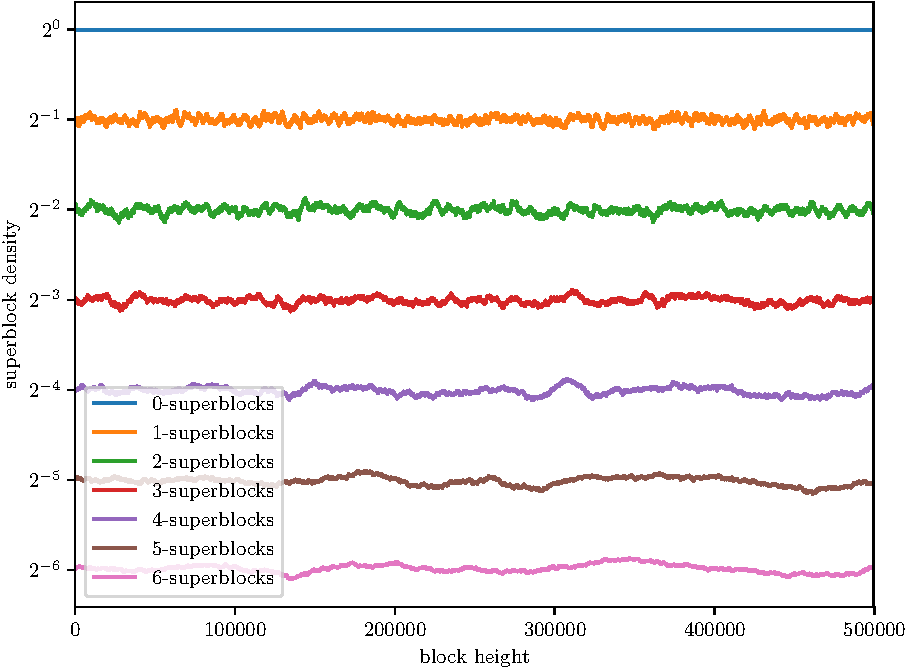
\includegraphics[width=0.95\textwidth]{figures/bitcoin-superblock-distribution.pdf}
  \caption{The distribution of block levels in Bitcoin and Bitcoin Cash. The
           graph has been corrected to account for variable difficulty. Block
           height in log-scale.}
  \label{fig.btc-bch-superblocks}
  \end{center}
\end{figure*}
